% !TEX root = ../swputhesis.tex
\chapter{相关技术及理论介绍}

\section{异常流量数据检测相关概念}
在网络流量异常检测领域的现有研究中，长尾分布下的数据不平衡问题与复杂环境
下的未知攻击检测是当前面临的两个核心挑战。

在长尾分布下的异常检测研究方面，传统的无监督单分类方法（如支持向量数据描
述、自编码器等）普遍基于正常流量在特征空间中紧凑分布的理想假设。然而，真
实网络中的正常流量往往呈现显著的长尾分布特性，即由海量高频的单一背景流量
构成“头部”，而由少量低频但多样的关键业务流量构成“尾部”。现有模型在优化
时不可避免地被高频头部样本主导，导致特征中心向高密度区域偏移，决策边界过
度收缩。这种偏差会使得处于长尾部分的稀疏正常流量被排斥在边界之外，从而引发极高的误报率。

在面向未知攻击的异常检测研究方面，随着零日攻击和高级持续性威胁的频发，异常
标签往往难以获取。现有的无监督聚类检测方法虽然在一定程度上摆脱了对标签的依
赖，但普遍存在单一聚类中心的理论局限。真实网络中的正常业务极其异构，往往表
现为多个独立的高密度聚集区。若强行使用单一中心拟合多中心的复杂分布，不仅会
造成处于分布边缘的合法样本被误报，更会导致潜伏在多类正常模式间隙的复杂未知
攻击成功逃避检测。


\subsection{数据包与PCAP接口}
数据包是计算机网络中进行数据传输的基本单位，它将用户需要传输的数据
与必要的控制信息（如地址、协议类型、校验信息等）按照协议规范组织在
一起，使数据能够在网络中被识别、传输、转发和接收。

\begin{figure}[h]
	\centering
	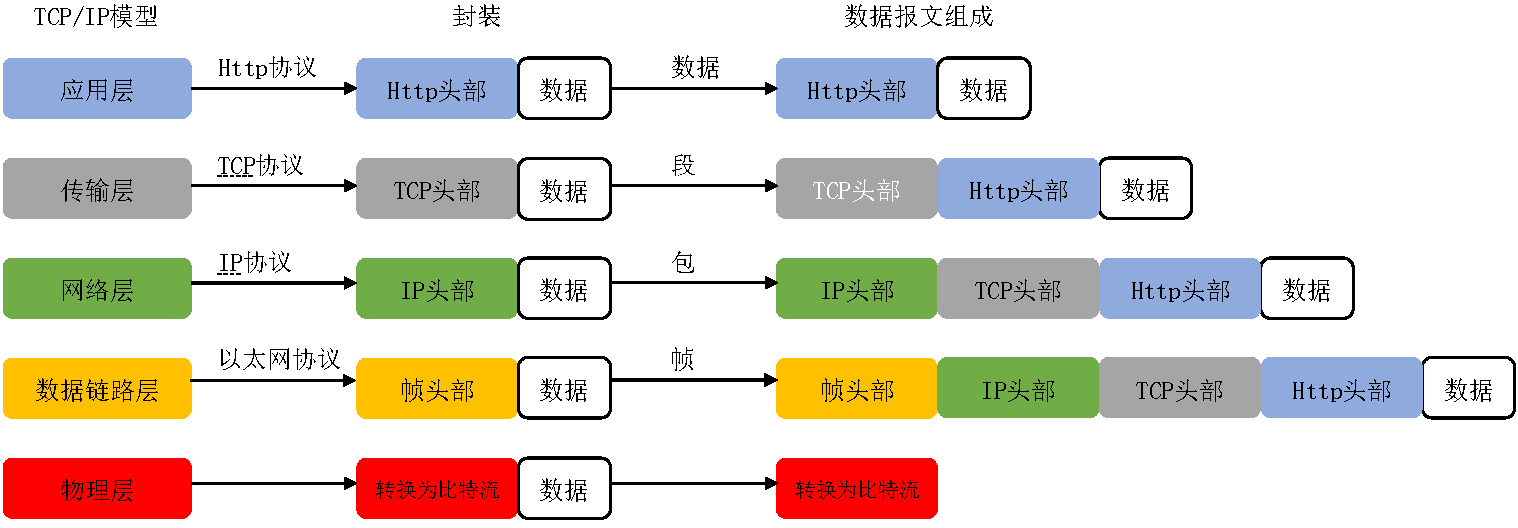
\includegraphics[scale=0.6]{fig/chapter2/数据封装过程.pdf}
	\caption{数据封装流程}
	\label{fig:2-1}
\end{figure}
在发送端，用户数据按照 TCP/IP 协议体系自上而下逐层封装：应用层对
数据进行初步封装；传输层将其封装为 TCP/UDP 数据段以实现端到端通
信；网络层加入 IP 头部形成 IP 数据包以完成路由；数据链路层将其封
装成帧；最终在物理层以比特流形式通过传输介质发送。数据封装的整体
流程如图\ref{fig:2-1}所示，主要包含五个步骤。

PCAP（Packet Capture）接口是一种用于捕获和存储网络数据包的标准化
接口与文件格式，广泛应用于网络监控、流量分析和网络安全研究等领域。它
能够在网络接口处拦截经过的数据包，并向上层应用提供统一的数据访问方式。
通过 PCAP 接口，网络监控工具（如 Wireshark、tcpdump）可以按照时间
顺序获取网络数据包，并支持使用过滤规则对流量进行筛选，从而提高捕获效率。
捕获到的数据通常以 PCAP 文件形式保存，文件由全局头和若干数据包记录组成，
每条记录包含数据包的时间戳、长度信息及原始数据内容，PCAP文件存储的信息格
式如图\ref{fig:2-2}所示。在网络异常流量检测中，PCAP 接口能够完整保留原始网络通信数
据，为后续的特征提取、行为分析和模型训练提供基础数据支持。

\begin{figure}[h]
	\centering
	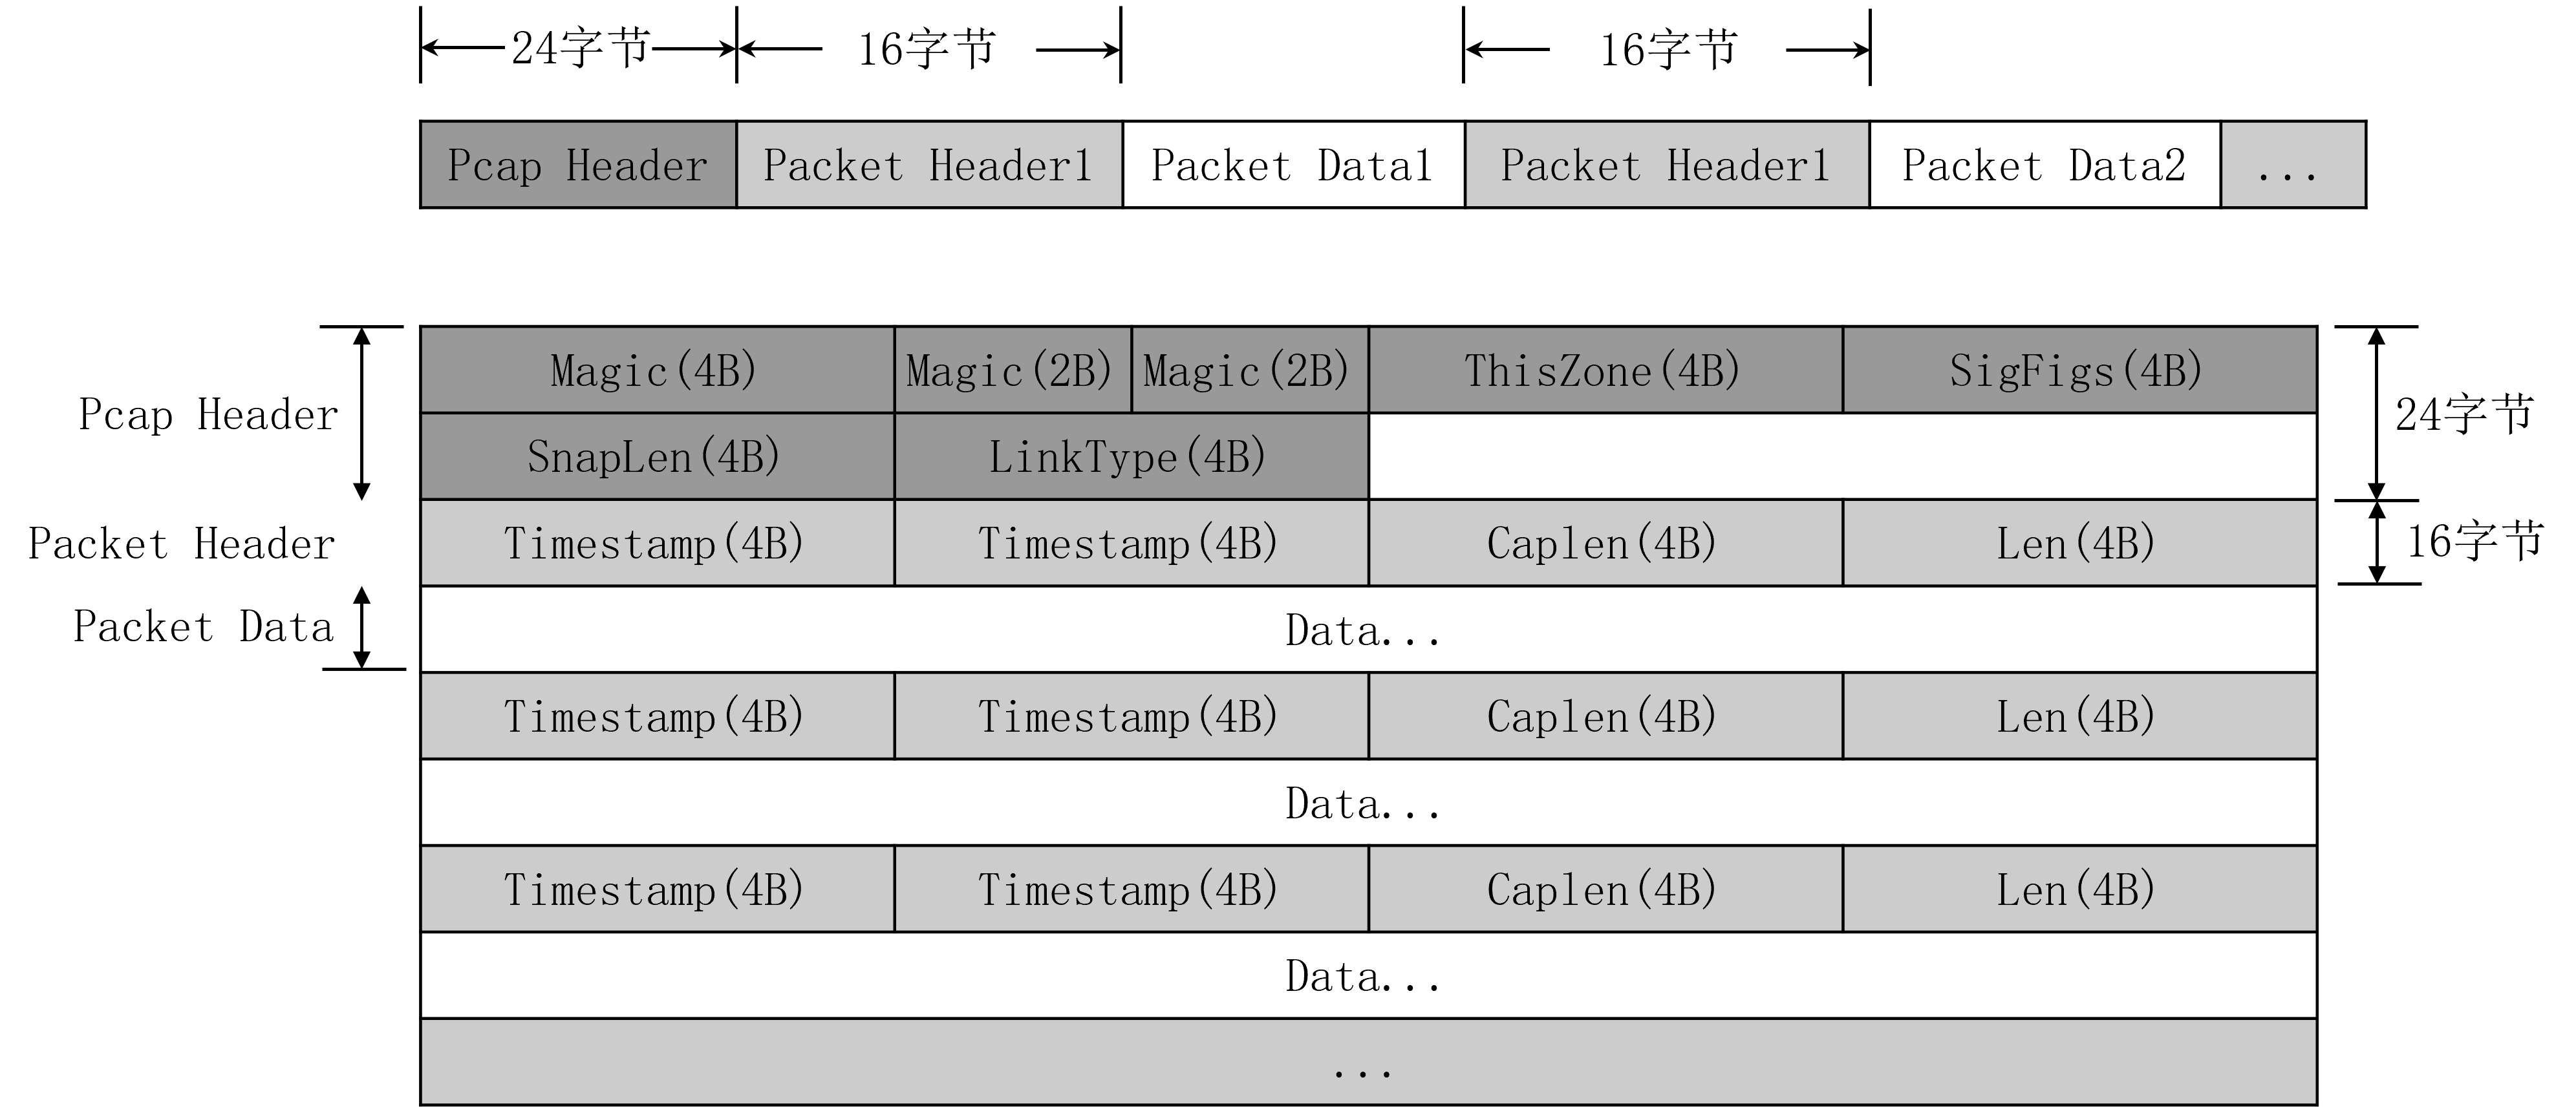
\includegraphics[scale=0.5]{fig/chapter2/PCAP文件结构.png}
	\caption{PCAP文件结构}
	\label{fig:2-2}
\end{figure}

\subsection{网络流量数据}
在网络通信中，数据包是数据传输的最小离散单位。由于单包包含的信息有限，且包与包之
间存在紧密的时序与通信关联，为更全面地刻画网络行为，研究通常以网络流作为基本分析
对象。网络流是指在特定时间窗口内，具有相同五元组（源IP、目的IP、源端口、目的端口
和传输层协议）的数据包集合\cite{1025069439.nh}。通过按五元组和时间顺序将离散数据包进行聚合，能够提取具
有明确语义的通信模式，准确反映主机间的交互特征，其聚合过程如图\ref{fig:2-3}所示。

\begin{figure}[h]
    \centering
    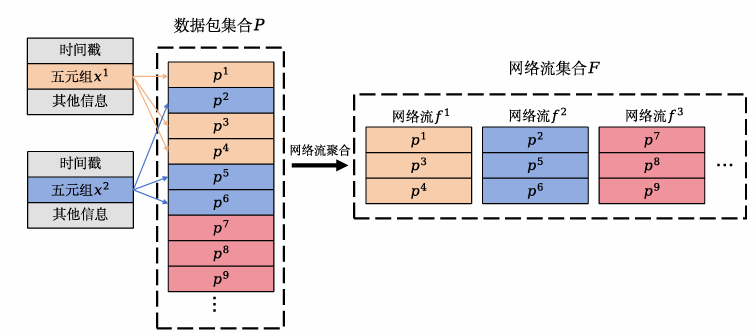
\includegraphics[scale=0.8]{fig/chapter2/网络流聚合过程.png}
    \caption{网络流聚合过程}
    \label{fig:2-3}
\end{figure}

假设某时间段内共收集了 $n$ 个数据包，可将其定义为数据包集合 $P$：

\begin{equation}
    \begin{gathered}
        P = \{p^1, p^2, \dots, p^n\} \\
        p^i = \{t^i, x^i, b^i\}, \quad i = 1, 2, \dots, n
    \end{gathered}
\end{equation}

其中，$p^i$ 表示第 $i$ 个数据包；$t^i$、$x^i$ 和 $b^i$ 分别代表该包被截获的时间戳、
五元组信息以及其他传输载荷信息。

经过网络流聚合后，离散的包集合 $P$ 被映射为包含 $m$ 条网络流的集合 $F$。每条网络
流 $f^i$ 由具有相同五元组 $x^i$ 的 $k$ 个数据包组成，并严格按时间戳递增排
序（$t^1 < t^2 < \dots < t^k$）：

\begin{equation}
\begin{gathered}
    F = \{f^1, f^2, \dots, f^m\} \\
    f^i = \{(t^1, x^i, b^1), (t^2, x^i, b^2), \dots, (t^k, x^i, b^k)\} \\
    m \le n, \quad k \le n
\end{gathered}
\end{equation}

由于总包数为 $n$，因此聚合后的网络流总数 $m$ 以及单条流内包含的数据包数量 $k$ 均不大于 $n$。

\subsection{网络攻击类型}
网络攻击是造成网络异常流量的主要原因之一。攻击行为在产生方式、通信模式以及资源消耗特征等
方面，均与正常用户访问存在显著差异，从而在网络流量中表现出明显的异常特征。根据攻击目标和
实现方式的不同，常见的网络攻击类型主要包括拒绝服务攻击、Web 攻击以及远程未授权访问攻击。

（1）拒绝服务攻击（Denial of Service，DoS）：
拒绝服务攻击通过向目标服务器持续发送大量伪造或恶意请求，占用系统计算资源、网络带宽或连接
队列，使服务器无法及时响应合法用户请求。此类攻击通常表现为流量规模突增、请求频率异常以及
连接状态异常堆积等特征，容易引发网络延迟增加、服务中断甚至系统崩溃。常见的拒绝服务攻击方
式包括 UDP 泛洪攻击、SYN 泛洪攻击以及 Land 攻击等，是异常流量检测研究中的典型攻击类型。

（2）Web 攻击：
Web 攻击主要针对 Web 应用程序及其后端服务器，利用程序设计缺陷或安全机制薄弱点实施恶意操
作。常见的 Web 攻击形式包括跨站脚本攻击（XSS）、SQL 注入和跨站请求伪造（CSRF）。此类攻
击不仅可能导致网页内容被篡改、用户会话被劫持，还可能造成数据库信息泄露或非法操作。从流量特
征角度看，Web 攻击往往表现为异常的请求参数、非正常访问路径以及请求行为模式的明显偏移。

（3）远程未授权访问攻击：
远程未授权访问攻击是指攻击者利用系统漏洞、弱口令或暴力破解等手段，在未获得合法授权的情况
下，通过远程登录方式（如 SSH、Telnet 等）侵入目标系统。一旦成功获取访问权限，攻击者可
能在受害者不知情的情况下执行数据窃取、恶意程序植入或系统控制等破坏性操作。该类攻击在网络
流量中通常表现为异常登录尝试频繁、访问时间和访问行为不符合正常用户使用习惯等特征。

\section{基于无监督学习的异常流量检测方法}
在网络安全防御体系中，由于获取带有精确标注的异常攻击样本成本高昂，且真实的流量环境
中不断涌现出未知的零日攻击，传统的有监督学习方法常常面临严重的泛化瓶颈。无监督学习
方法因其无需依赖先验标签，能够直接从海量的原始网络流量中挖掘正常行为的内在分布规律
，并将显著偏离该正常模式的流量判定为异常。这种“非正常即异常”的检测范式赋予了模型发
现未知威胁的能力。现有的无监督异常流量检测方法按照底层机制的不同，主要可划分为基于
聚类、基于边界、基于隔离以及基于深度重构四大类\cite{kozik2024survey}。

\subsection{基于聚类的检测方法}
基于聚类的检测方法是无监督异常检测中最为经典的分支\cite{kakade2024network}。
该类方法的核心假设是正常流量在特征空间中具有高度的相似性，通常会形成一个或多个高密
度的聚集类簇，而异常攻击流量则表现为游离于大类簇之外的离群点或孤立的小规模微簇。代
表性算法包括 K-Means、DBSCAN 以及高斯混合模型等，它们通过计算样本间的距离或相似
度进行无监督划分，具有较强的可解释性。然而，传统聚类算法在面对高维网络流量时容易陷
入维度灾难，且难以自适应地确定最佳的类簇数量与密度判定阈值。

为了克服单一聚类中心在复杂网络环境下的理论局限性，多中心无监督聚类建模思想被提出并广
泛应用\cite{wu2024unsupervised}。真实网络中的正常业务极其异构，该思想通过引入多
个聚类中心集合：
$$ \mathcal{E} = \{ \mathbf{e}_1, \mathbf{e}_2, \ldots, \mathbf{e}_M \} $$
以多个潜在正常行为模式共同刻画正常流量的整体分布。在这一框架下，正常样本通常至少与某一聚类
中心保持较小距离，聚集在多个相对独立或部分重叠的区域内；而异常样本则往往同时远离所有聚类中
心。这种多中心结构有效缓解了单中心模型在复杂分布下容易导致的误报与漏报问题，为更精准的异常
判别奠定了数学基础。
为更直观地说明多中心无监督聚类建模思想，图\ref{fig:无监督多中心聚类方法示意图}
给出了该方法在二维特征空间中的示意图。
如图所示，蓝色圆点表示模型学习得到的多个正常行为模式聚类中心：
\begin{figure}[h]
	\centering
	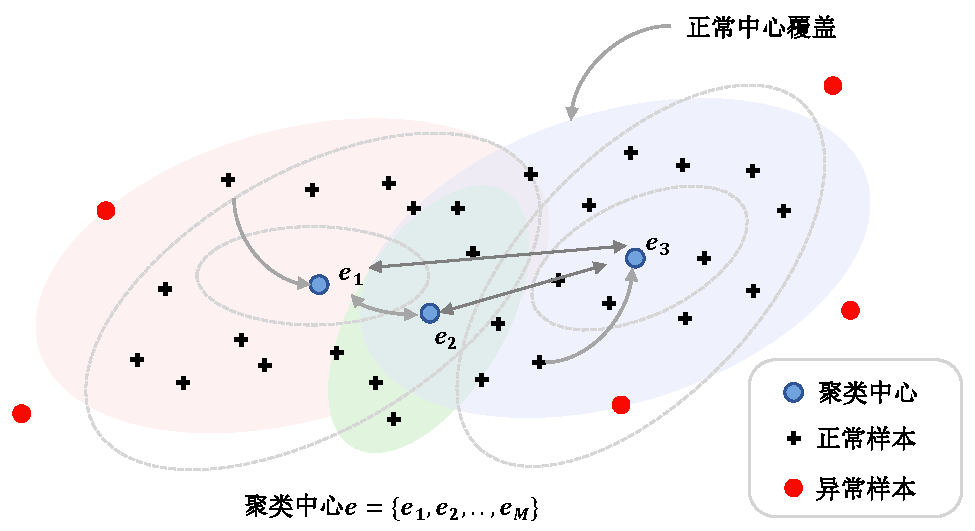
\includegraphics[scale=0.7]{fig/chapter4/多中心聚类方法示意图.pdf}
	\caption{无监督多中心聚类方法示意图}
	\label{fig:无监督多中心聚类方法示意图}
\end{figure}

\subsection{基于边界的检测方法}
基于边界的检测方法旨在特征空间中构建一个尽可能紧凑的闭合决策边界或包络面，将绝大多数的正常
流量样本包裹在边界内部，在推理阶段落在该边界之外的新样本即被判定为异常。典型的代表算法包括
单分类支持向量机与支持向量数据描述\cite{gondim2023applying}。这类方法具备坚实的统计学
习理论基础，并可通过核技巧有效处理数据的非线性映射问题。但在面对具有显著长尾分布特性或极端
不平衡的海量网络流量时，其寻优过程容易被高频的单一正常模式主导，导致决策边界过度收缩或发生
偏移，从而难以兼顾处于长尾部分的低频稀疏正常业务流。

\subsection{基于距离的检测方法}
基于距离与隔离的检测方法主要利用了异常数据在统计学和空间分布上“少且不同”的本质特征。
例如，孤立森林及其针对高维与时序流数据的隔离变体\cite{yepmo2024leveraging}，通
过随机选择特征维度与设定切分值来构建隔离树，使得分布在边缘区域的异常流量因较短的平均
路径长度而被迅速孤立。此类方法无需计算复杂的全局距离，具有极低的线性时间复杂度，非常
适合大规模流式网络数据的实时处理\cite{maspo2026anomaly}，但难以有效捕获深层的时序依赖。

在距离度量领域，为了更准确地刻画样本在特征空间中的分布状态并处理不平衡数据，实例欧氏距离（IED）
常被作为量化局部密度特征的核心工具。对于给定样本 $x_i$，其 IED 值定义为该样本与其在特征空间
中 $k$ 个最近邻样本的平均欧氏距离\cite{pang2025imbalanced}。其数学表达式如下：
$$ D_{IED}(x_i) = \frac{1}{k} \sum_{x_j \in \mathcal{N}_k(x_i)} \left\| \phi(x_i) - \phi(x_j) \right\|_2 $$
其中，$\mathcal{N}_k(x_i)$ 表示样本 $x_i$ 在特征空间中的 $k$ 近邻集合，$\phi(\cdot)$ 
为将原始数据映射到隐层空间的特征表示函数。

IED 值直接反映了样本的局部空间密度：低 IED 值对应位于密集中心的高频“头部”正常流量；高 IED 值则
对应位于稀疏边缘地带的多样化“长尾”正常模式。这一客观量化指标为在完全无监督条件下评估样本稀缺性、动
态调整模型训练权重提供了可靠的标准。

\subsection{基于深度重构的检测方法}
基于深度重构的检测方法随着现代神经网络的发展已逐渐成为当前学术界的研究主流\cite{jian2023robust}。
此类方法主要利用自编码器、变分自编码器或生成对抗网络等深度架构，在无标签的正常流量数据上进行表征压
缩与重建训练\cite{bahlali2025self,zhang2024unsupervised}。模型被迫学习正常流量的高阶非线性
特征与底层低维流形结构。在实际检测阶段，由于模型仅掌握了正常模式的重构规律，当输入未见过的异常攻击
流量时，网络往往无法完美还原输入，从而产生显著偏高的重构误差。此类方法在处理高维、高并发以及复杂
异构的网络流量方面展现出了卓越的表征学习能力。

\section{本章小结}
本章主要介绍了网络异常流量检测涉及的相关基础概念与核心检测理论。首先，深入分析了
当前异常检测领域面临的两大核心挑战：长尾分布下的数据不平衡问题与复杂环境下的未知
攻击检测问题。随后，从底层数据出发，详细阐述了数据包的封装过程、PCAP 接口的捕获
机制，以及离散数据包向网络流聚合的数学表达，为后续的特征提取与模型训练提供了数据
层面的理论基础。同时，梳理了导致网络异常的典型攻击类型，包括拒绝服务攻击、Web 
攻击和远程未授权访问攻击及其流量特征。

在此基础上，本章重点探讨了基于无监督学习的异常流量检测方法，将其系统划分为基于聚类、
基于边界、基于距离以及基于深度重构四大主流分支，并客观分析了各类方法的优势与局限性。
针对真实网络流量中呈现的复杂异构分布与长尾特性，本章进一步详细论述了多中心无监督聚
类建模思想以及基于实例欧氏距离（IED）的局部密度度量理论。这两项理论的引入，有效弥补
了传统单分类或单中心模型在处理高频背景流量与低频稀疏正常业务时的缺陷，为后续章节中解
决未知攻击检测和长尾数据不平衡问题奠定了坚实的数学与理论基础。